%% ma: L12-B13-0004
%% lop: 12
%% chuong: 4
%% bai: 13
%% dang: 12.13.3
%% loai: TLN
%% muc: VD
%% dap_an: "3200"
%% nguon: "0. ĐỀ THAM KHẢO TN THPT 2025.pdf (D00), Phần III Câu 4"
%% kien_thuc: "Bài 13 (diện tích hình phẳng giới hạn bởi parabol và trục hoành), lập phương trình parabol từ ba điểm (Lớp 10 Bài 16)"
%% trang_thai: cho-duyet
%% ly_do: "Dạng toán mới đề xuất 12.13.3, chờ giáo viên duyệt"
\begin{ex}
Kiến trúc sư thiết kế một khu sinh hoạt cộng đồng có dạng hình chữ nhật với chiều rộng và chiều dài lần lượt là $60$ m và $80$ m. Trong đó, phần được tô màu đậm là sân chơi, phần còn lại để trồng hoa. Mỗi phần trồng hoa có đường biên cong là một phần của parabol với đỉnh thuộc một trục đối xứng của hình chữ nhật và khoảng cách từ đỉnh đó đến trung điểm cạnh tương ứng của hình chữ nhật bằng $20$ m (xem hình minh họa). Diện tích của phần sân chơi là bao nhiêu mét vuông?
\begin{center}
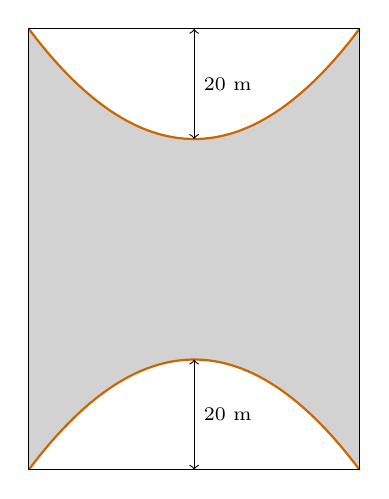
\begin{tikzpicture}[scale=.07]
  \fill[gray!35] (0,0) rectangle (60,80);
  \fill[white] (0,0) -- plot[domain=0:60,samples=60] (\x,{-\x*\x/45+4*\x/3}) -- cycle;
  \fill[white] (0,80) -- plot[domain=0:60,samples=60] (\x,{80+\x*\x/45-4*\x/3}) -- cycle;
  \draw[orange!80!black,thick,domain=0:60,samples=60] plot (\x,{-\x*\x/45+4*\x/3});
  \draw[orange!80!black,thick,domain=0:60,samples=60] plot (\x,{80+\x*\x/45-4*\x/3});
  \draw (0,0) rectangle (60,80);
  \draw[<->] (30,0)--(30,20) node[midway,right,font=\scriptsize]{$20$ m};
  \draw[<->] (30,80)--(30,60) node[midway,right,font=\scriptsize]{$20$ m};
\end{tikzpicture}
\end{center}
\shortans{3200}
\loigiai{Chọn hệ trục $Oxy$ với $O$ là một đỉnh của hình chữ nhật, $Ox$ theo cạnh $60$ m. Parabol phía dưới đi qua $O(0;0)$, $I(30;20)$, $A(60;0)$ nên có phương trình $y=-\dfrac{1}{45}x^2+\dfrac43x$.
Diện tích mỗi phần trồng hoa $S_h=\displaystyle\int_0^{60}\left(-\frac{x^2}{45}+\frac{4x}{3}\right)\mathrm dx=800\ \mathrm{m^2}$; hai phần bằng nhau (đối xứng).
Diện tích sân chơi $S=60\cdot80-2\cdot800=3200\ \mathrm{m^2}$.}
\end{ex}
